During the thesis a lot of various experiments were conducted that required different configurations of the telescope. In the next chapters these set-up are briefly summarised and sorted by complexity. 
% ========================================================
% SINGLE CHIP
% ========================================================
\section{Single \ac{ROC} Assembly}
The single \ac{ROC} set-up  is very important for basic functionality tests of a \ac{ROC} and for the general understanding of the chip. A real set-up a shown in \ar{psingleroc} and a general schematic drawn in \ar{psinglerocdraw}. It is possible to either connect an adapter plane directly to the \ac{ROC} or equip the telescope with a single plane and use jumpers at the vacant positions.
\begin{figure}[ht]
	\centering
	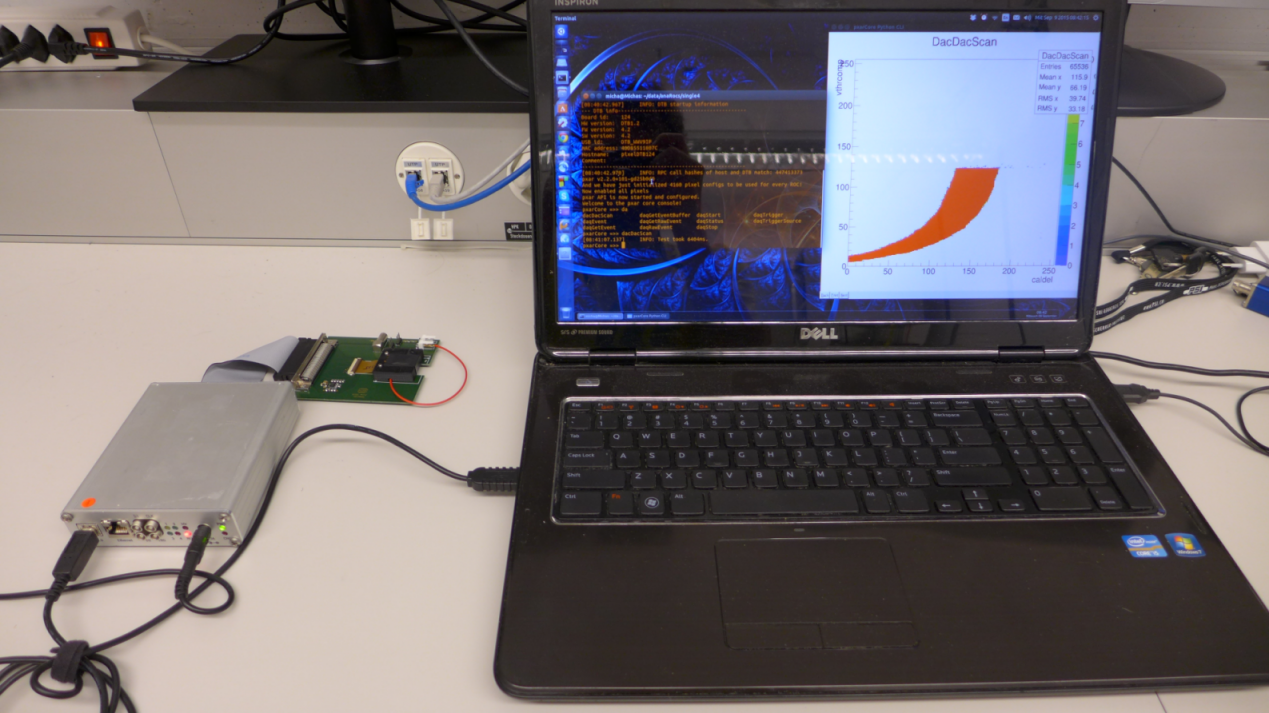
\includegraphics[width=0.95\textwidth]{setup/singlesetup}
	\caption{A single adapter plane operated with a \ac{DTB} connected to a laptop.}
	\label{psingleroc}
\end{figure}\no
\begin{figure}[ht]
	\centering
	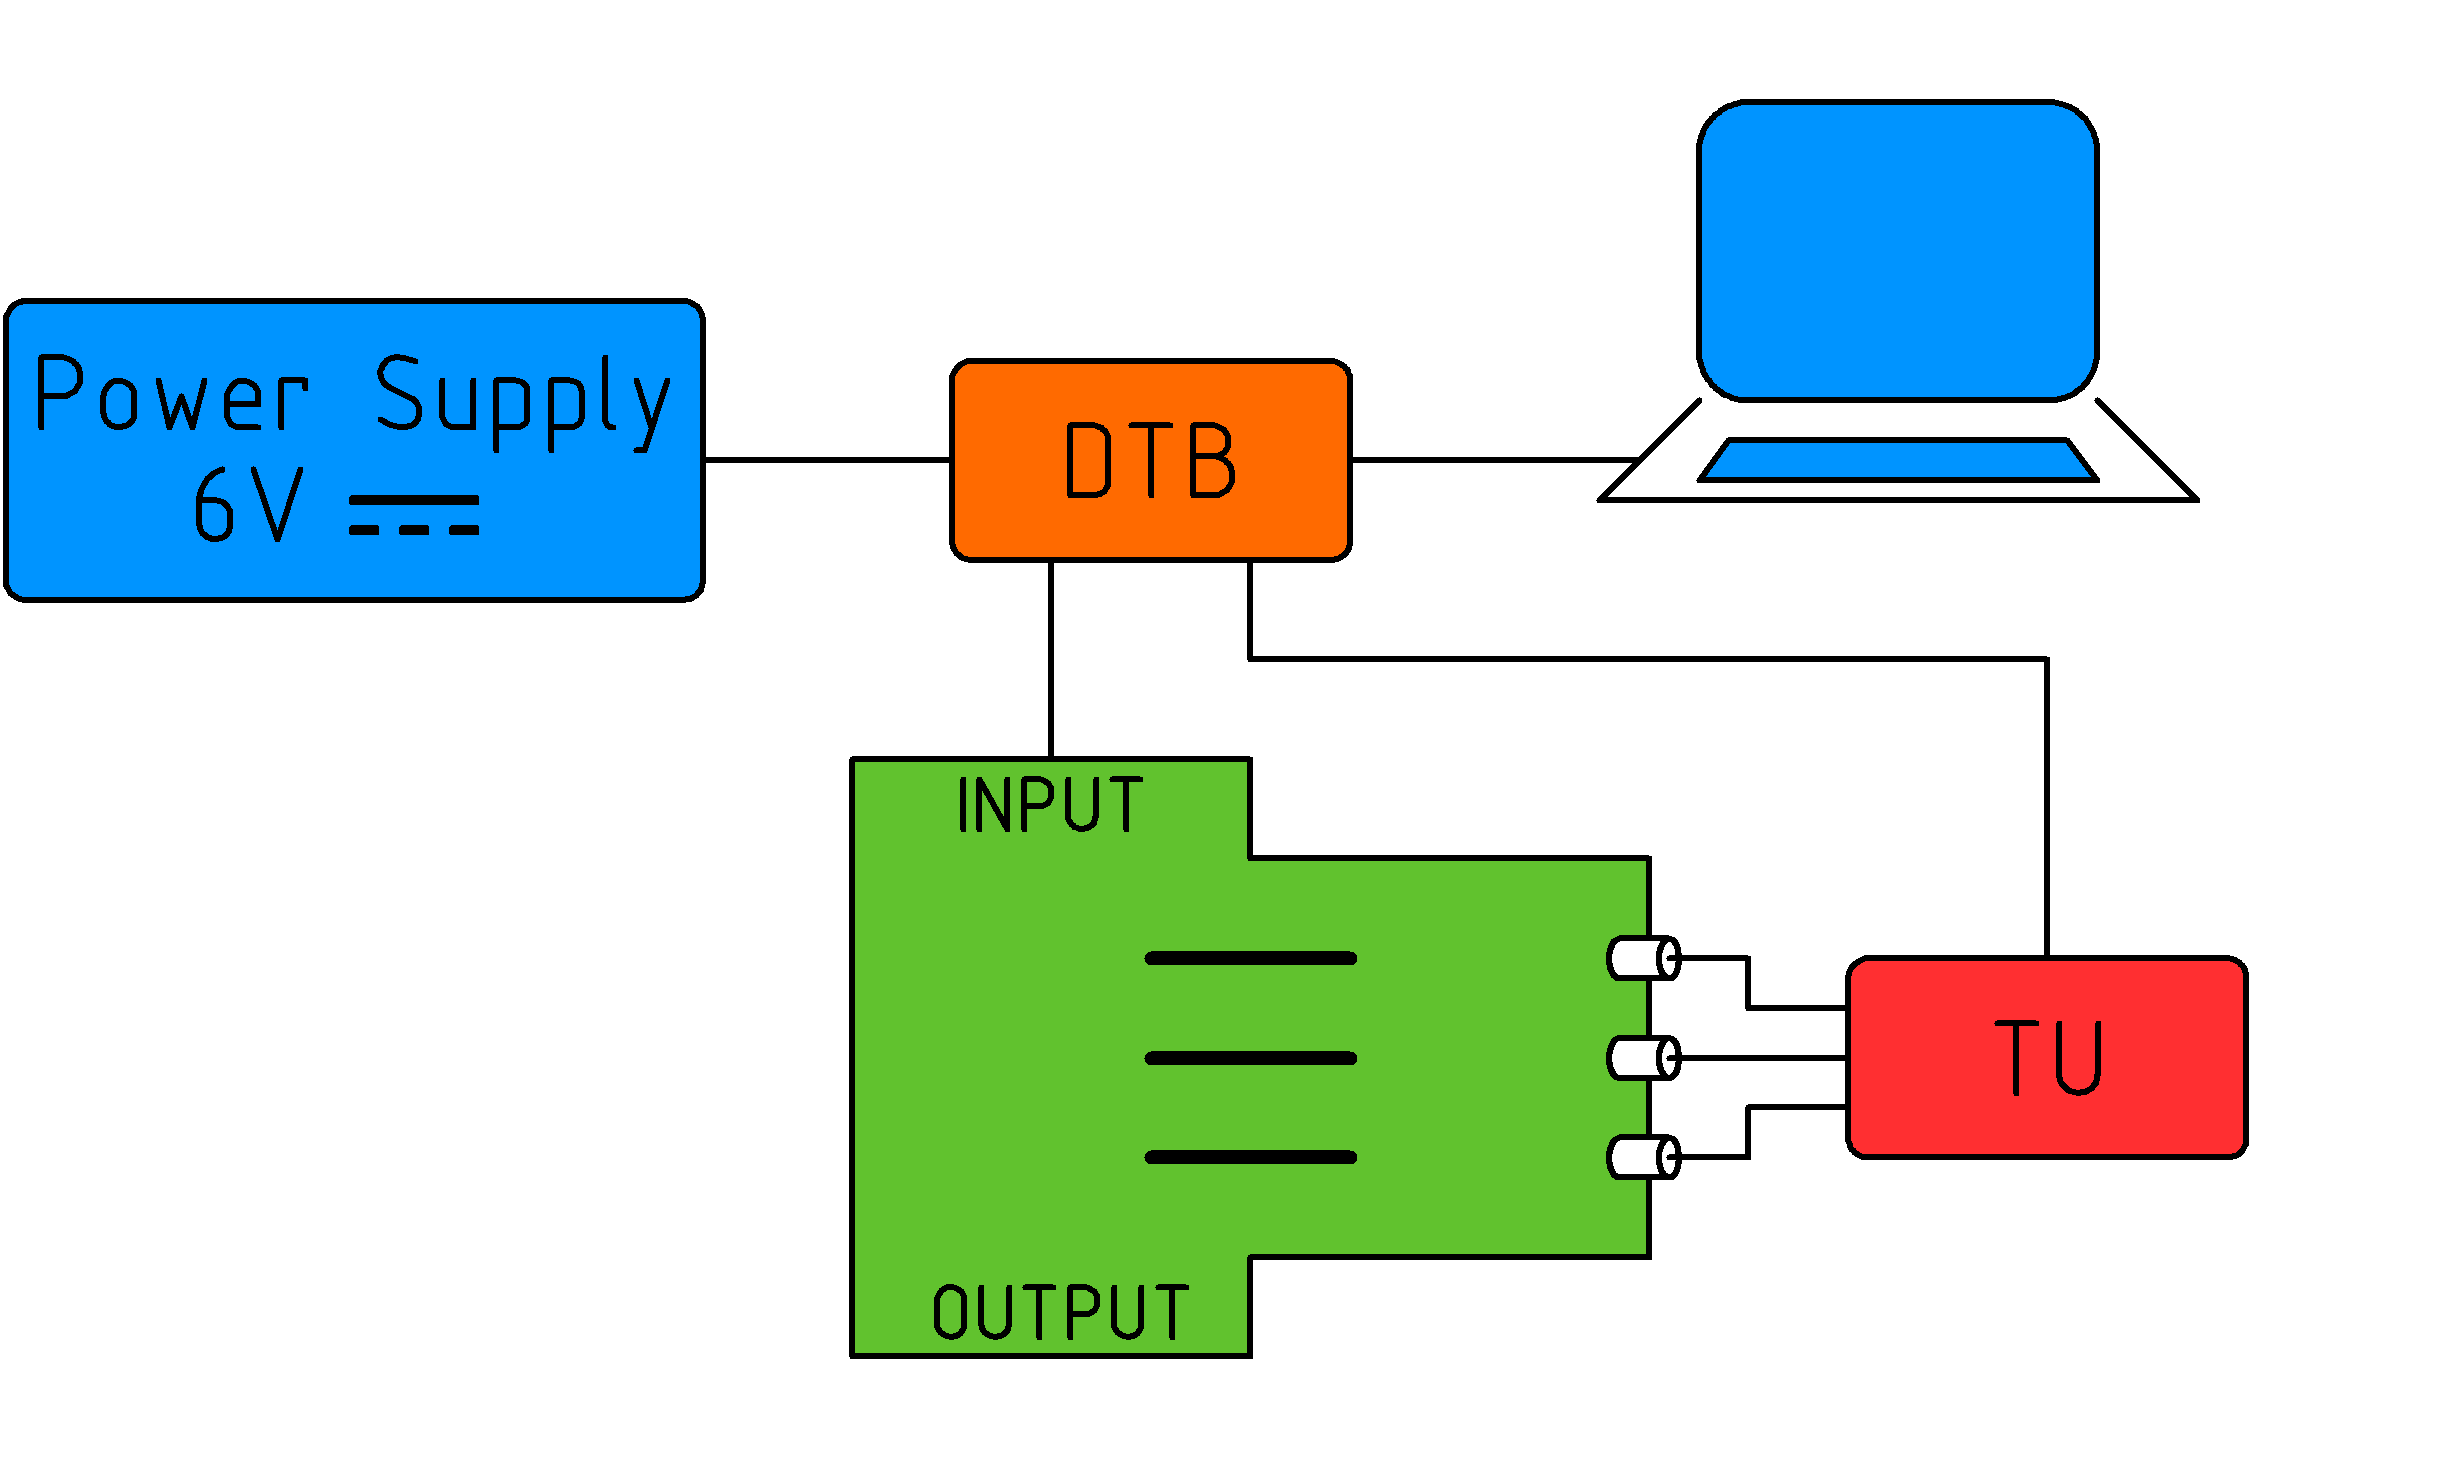
\includegraphics[width=0.6\textwidth]{singletel}
	\caption{Schematics of a single telescope set-up.}
	\label{psinglerocdraw}
\end{figure}\no
% ========================================================
\subsection{Simple Testing Set-up}
The most minimalistic set-up consists out of a single \ac{ROC}, the \ac{DTB} and a computer. It used for testing purposes using calibrate signals. Thus, it requires no external trigger source and the \ac{TU} in \ar{psinglerocdraw} is not required.
% ========================================================
\subsection{Source and External Trigger}
The above set-up can be extended with an external trigger. For almost every set-up\footnote{Exceptions are mentioned in \ar{sexp}} the fast-OR of the analogue \ac{ROC}s is used as trigger. Thus, the one plane set-up with external self trigger is only viable for the analogue chips.\\
In order to create particle hits, a radioactive \chemfig{Sr^{90}} source can be placed on top the \ac{ROC}. Thereby fast-ORs are generated which have to be sent back to the \ac{ROC} using the trigger logic in \ar{plogic1}. In this case with only one plane the coincidence unit is not required.
% ========================================================
\subsection{Trigger Logic}\label{striglog1}
The fast-ORs leaving the planes are differential signals, which is why their base line has a zero offset. Since we are using NIM the negative part of the differential signal is chosen and sent to a self made level shifter that shifts the baseline to zero. In order to transform the signal into a rectangular NIM pulse a discriminator is used next. This is done for the fast-ORs of all available planes in parallel. Every signal on its own is sent to a scaler to count the number of events for each plane. All signals together are sent to a coincidence unit, where the user can decide which effective trigger is used. It is possible, for example, to select only events with triggers in every plane by putting all fast-ORs in coincidence or to use only the trigger from a single plane and discard the rest. Afterwards the effective trigger rate is counted by a scaler. In a last step the effective trigger is converted into a \ac{TTL} signal by a \ac{TTL} converter. The signals is then distributed back to the planes via the \ac{DTB}.
\begin{figure}[ht]
	\centering
	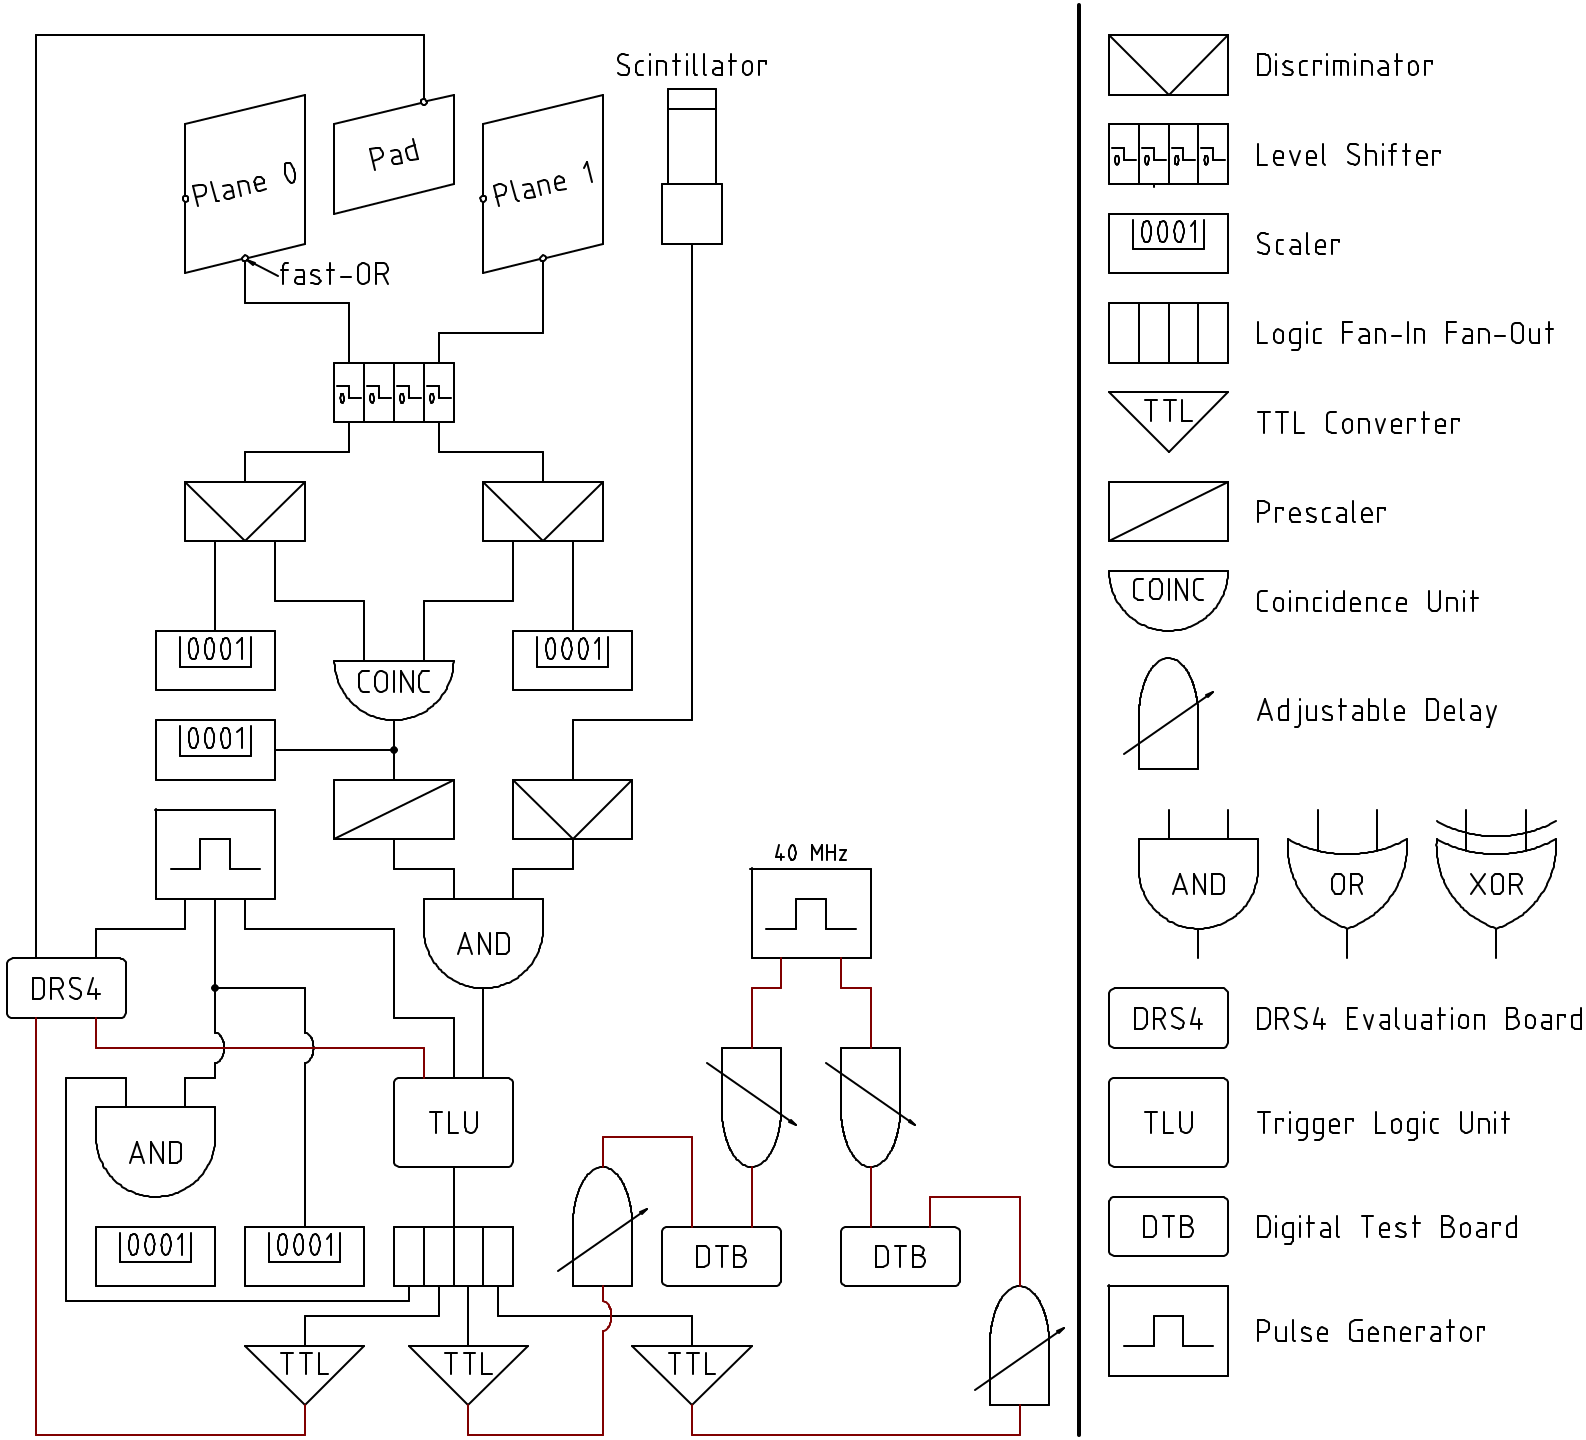
\includegraphics[width=0.6\textwidth]{triglog1}
	\caption{Simple trigger logic for a testing set-up. The number of planes may differ from the example, two was chosen for demonstration. To simplify matters, the connection from the \ac{DTB} to the planes is left out.}
	\label{plogic1}
\end{figure}\no
% ========================================================
% TELESCOPE
% ========================================================
\section{Single Telescope Set-up}
The single telescope set-up refers to a configuration with more than one plane in a single telescope controlled by a \ac{DTB}. Is very useful for the commissioning of the telescope using calibrate signals. Different numbers of planes can be tested. For external triggers the same logic as in \ar{striglog1} applies. However, the self trigger mode with a source is not possible for more than two planes because the beta electrons generally do not have enough energy to produce hits in more than two planes. A configuration with three planes is shown in \ar{p3plane}.
\begin{figure}[ht]
	\centering
	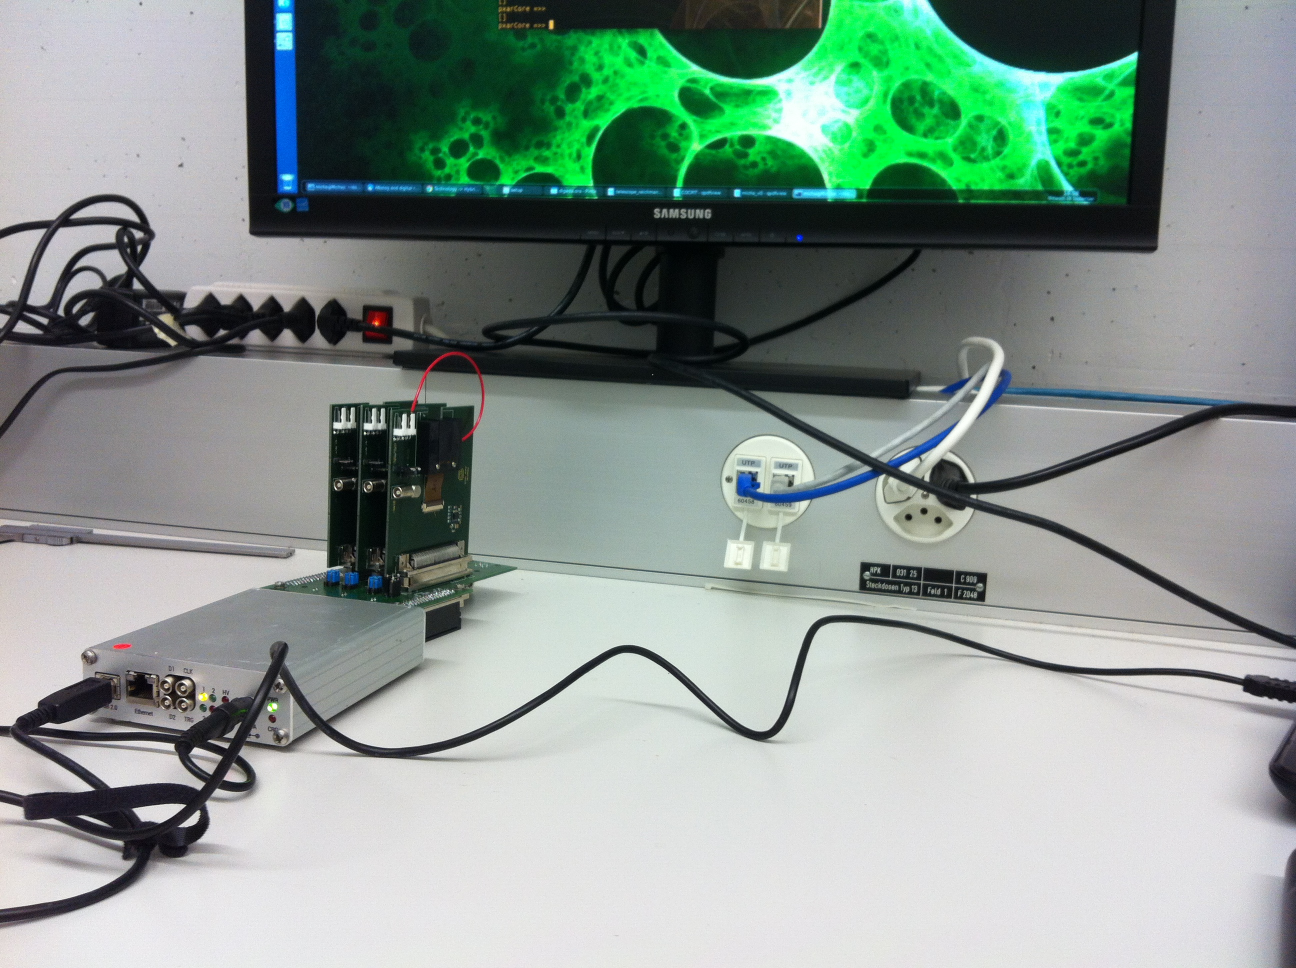
\includegraphics[width=0.95\textwidth]{3planetel}
	\caption{Telescope configured with three planes.}
	\label{p3plane}
\end{figure}\no
% ========================================================
% BEAM TEST
% ========================================================
\section{Beam Test Set-up}
In order to use the telescope to its full extent is has to placed inside of a particle beam of an accelerator. Being put there the telescope can be utilised on its own for debugging in self trigger mode with available fast-ORs for every single analogue plane. But the most important thing is to use it for its main purpose as auxiliary device for various \ac{DUT}s. A schematic visualisation of this set-up is shown in \ar{pfulldraw}. Every \ac{DUT} is placed inside a maximum number of six analogue planes that form a single telescope and are connected one \ac{DTB}. The trigger for all devices is the fast-OR of these analogue planes, which is handled by the trigger logic in \ar{plogic2}. During the beam tests for data taking usually two analogue were used in the front and the back adding up to a total number of four. The effective trigger almost always was a coincidence of the two inner planes, closest to the \ac{DUT}. The plastic scintillator at the end of the telescope is an optional device that used to get precise timing information about the particles; its signal is also fed to the trigger logic.\\
The examined types of \ac{DUT}s and their configuration within the telescope are named in the following:
\begin{itemize}
	\item one or two diamond pad detectors
	\item digital CMS pixel chips (silicon)
	\item digital CMS pixel chips with diamond as sensors
	\item pads combined with digital chips
	\item diamond and digital chips
\end{itemize}
The diamond pad detectors are made out of a single diamond sensor, whose signal is amplified and continuously read out by a DRS4 evaluation board. Digital and diamond pixel chips are placed inside the digital adapter planes and plugged into a motherboard which is controlled by a second \ac{DTB}. Two examples of these set-ups are shown out of different perspectives in \ar{sdut1} and \ar{sdut2}.
\begin{figure}[ht]
	\centering
	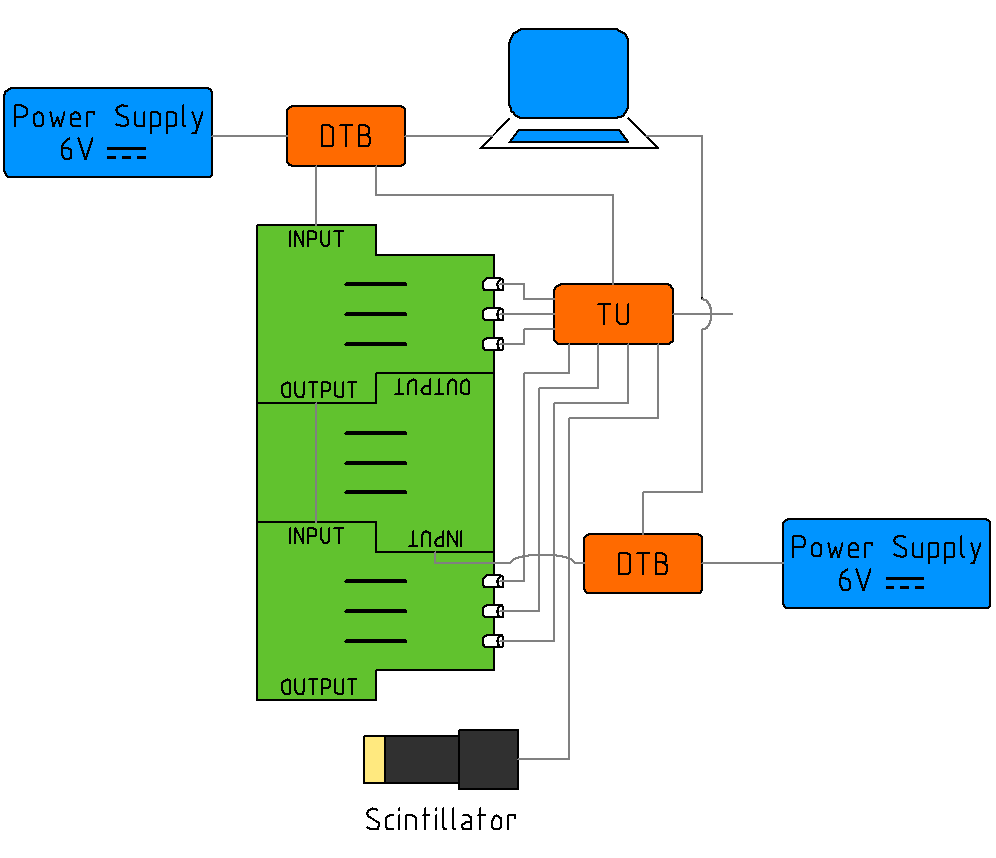
\includegraphics[width=0.9\textwidth]{felltel1}
	\caption{Schematics of a beam test set-up. The cables are drawn in grey to avoid confusion. To the open cable of the \ac{TU} may be connected to other devices like the DRS4 or a pulse generator. In this example a digital telescope is used as \ac{DUT} and placed between analogue planes. The two outer motherboards, which hold analogue planes are connected to each other and server a single telescope.}
	\label{pfulldraw}
\end{figure}\no
% ========================================================
\subsection{Trigger Logic}
The first part of the trigger logic for the beam test set-up is identical to the one described in \ar{striglog1}. Once the fast-ORs pass the coincidence unit there is a pre-scaling option to reduce the effective trigger rate. The effective trigger can then be brought into coincidence with a discriminated and delayable trigger signal from a scintillator. The scintillator delivers very precise timing information about the detected particles, which is used to determine the timing of a fast-OR trigger within one bunch crossing. The coincided signal is then sent together with two additional signals to a device called \ac{TLU}. The other two signal are the BUSY signal of the DRS4 that indicates a particle detection in the pad detector and a tunable clock from a pulse generator that is used as reference signal for the DRS4. If another \ac{DUT} than a pad is in use, the BUSY signal may be generated by the effective trigger itself.\\
The \ac{TLU} is a device especially built for beam test applications. Its main purpose is the exact distribution of trigger signals to the devices, synchronised with the data-taking software. Therefore it has a programmable a logic inside. For our purposes it makes an logic OR with the pulser and the effective trigger of the fast-ORs and the scintillator. Depending on the pulse length of the BUSY signal the \ac{TLU} will not send triggers once such a signal is received. In case of pad detectors this is required due to the dead time that arises when the DRS4 is processing an event.\\
The trigger that leaves the \ac{TLU} is then split by a fan-in fan-out and distributed to all the data-taking devices. \\
For the case of running with analogue and digital planes and respectively two \ac{DTB}s there is small extension. In order to synchronise the two \ac{DTB}s, a common clock that can be delayed for both of the boards, is sent to their external clock inputs. There is also the option to delay the trigger to each of the \ac{DTB}s. These four delays can then be used to optimise the trigger timing and the event alignment between the two boards. It therefore can improve the event yield.\\
In the future it is planned to use a \ac{TU} that unifies all the functions above, including the abilities of the \ac{TLU}, into a single device. It is currently under test at the Ohio State University. For this thesis everything was built using NIM modules in combination with the \ac{TLU}.
\begin{figure}[ht]
	\centering
	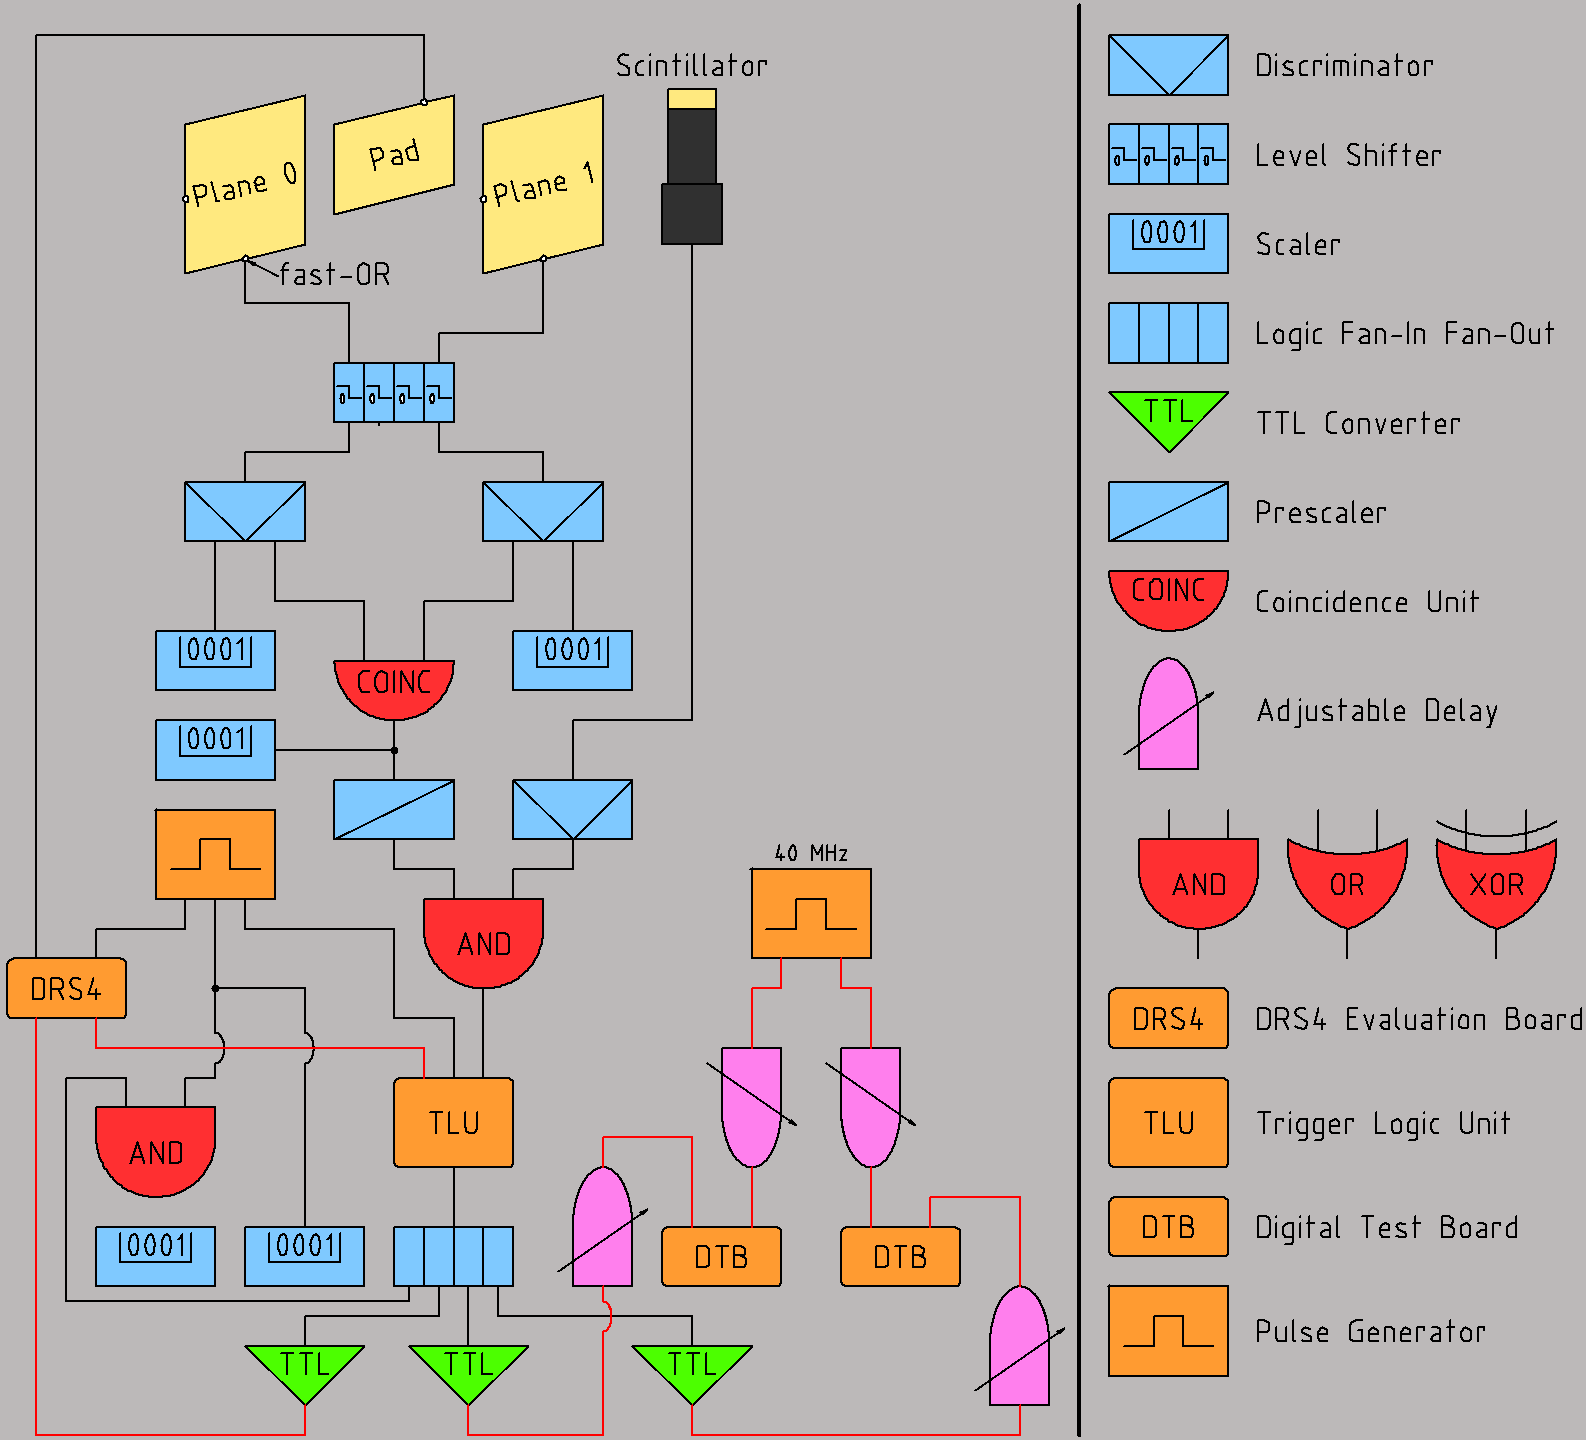
\includegraphics[width=0.95\textwidth]{triglog2}
	\caption{Full trigger logic. The pad may be exchanged with diamond pixels or other \ac{DUT}s. To simplify matters, the connection from the \ac{DTB} to the planes is left out. \ac{TTL} signal lines are drawn with red lines. The number of planes can also differ from this example.}
	\label{plogic2}
\end{figure}\no
\begin{figure}[ht]
	\centering
	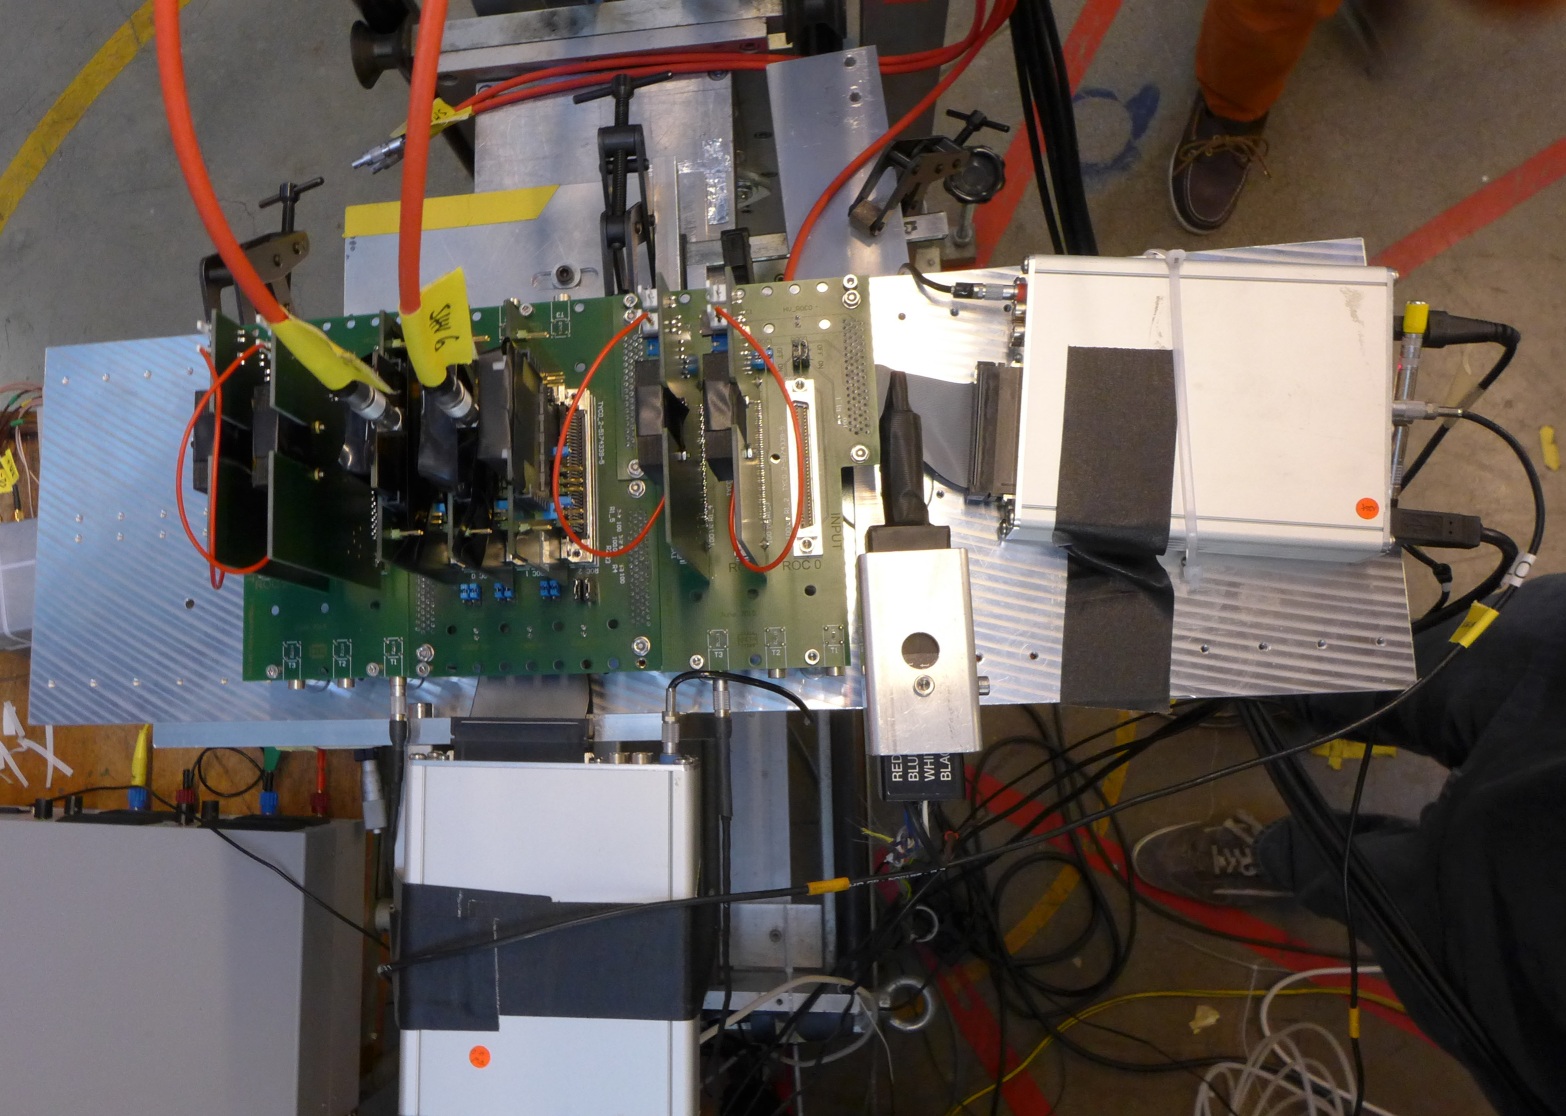
\includegraphics[width=0.95\textwidth]{setup/fullsetup}
	\caption{Top view of a beam test set-up at \ac{PSI}, the beam is coming from the left edge of the picture. The beam first hits two analogue planes on the first motherboard, afterwards two diamond pixel detectors and a digital silicon detectors on the next motherboard and then two analogue chips on a third motherboard. Last in line is a plastic scintillator. The four analogue chips are connected to the \ac{DTB} on the right side of the picture and the three digital chips to the test board in the front.}
	\label{sdut1}
\end{figure}\no
\begin{figure}[ht]
	\centering
	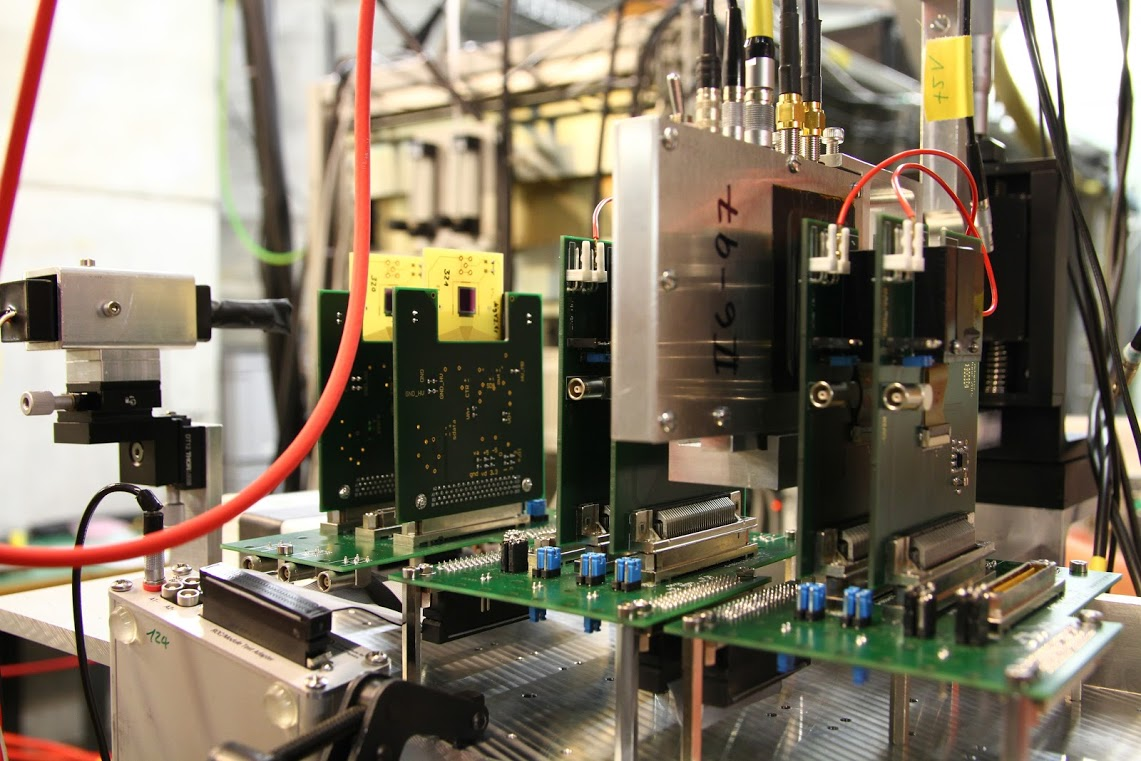
\includegraphics[width=0.95\textwidth]{setup/fullsetup1}
	\caption{Side view of beam test set-up at \ac{PSI}, the beam is coming from the right edge of the picture. The beam consecutively hits two analogue planes, a diamond pad detector and again two analogue planes. As mentioned before, the four analogue planes build one telescope. In the back are two digital silicon planes and a plastic scintillator, that were not used during this set-up.}
	\label{sdut2}
\end{figure}\no
% ========================================================
